


%% Future work
For future work, we intend to characterize the distribution of the most reputable research departments in CS worldwide, on a per subarea basis. We also want to do a temporal analysis of the evolution of the CS subareas communities over the last decades. Another further study is to validate the reputation model in other broad areas than CS, such as Economics, whose differences in publication patterns on a per subarea basis seem to be greater than in Computer Science.


%% Weighted normalized P-scores 
Weighted normalized P-scores allow identifying key venues for each subarea of knowledge with higher precision than alternatives such as global P-scores and citation-based metrics, see results in \cite{ueda17ictir}. They also provide for more accurate rankings of research groups on a per subarea basis, which we use to analyze the productivity of Brazilian graduate programs, in this work.


%% P-score proposal
Therefore, the reputation of a research group is strongly influenced by the reputation of its members, which is largely dependent on their publication records.

Once a reference group is selected, the reputation of its members is transferred to the venues. Recursively, since the reputation of research groups is strongly influenced by the reputation of the venues in which they published, the venues also transfer reputation to the groups.


%% Original Figure Group -> Group
\begin{figure}[h]
  \label{fig:groups-venues}
  \centering \small
  \def\x{\begin{array}{c}x\\x\end{array}}
  \(
  \let\svarraycolsep\arraycolsep
  \renewcommand\arraystretch{1.4}
  \begin{array}{c}
   \\
   {\scriptstyle Group}\\
   {\scriptstyle Venue}\\
  \\
  \end{array}
  \begin{array}{c}
   \\
   \scalerel*[1.5ex]{[}{\x}\\
  \\
  \end{array}
  \begin{array}{c}
   {\scriptstyle Group}\\
   Group \rightarrow Group \\
   Venue  \rightarrow Group \\
  \\
  \end{array}
  \begin{array}{c}
   {\scriptstyle Venue}\\
   Group  \rightarrow Venue \\
   Venue   \rightarrow Venue \\
  \\
  \end{array}
  \begin{array}{c}
   \\
   \scalerel*[1.5ex]{]}{\x}\\
  \\
  \end{array}
  \mathrm{}
  \arraycolsep\svarraycolsep
  \renewcommand\arraystretch{1.0}
  \)
  %\vspace{-0.6cm}
  \caption{Reputation flows between groups and venues.}
\end{figure}


%% P = Group --> Group...
\begin{align}\label{eq:newp}
%\[
\bP =
\left[
\begin{array}{r | r}
\ Group \rightarrow Group \ \ & \ Group \rightarrow Venue\ \\
\hline
\ Venue \rightarrow Group \ \ & \ Venue \rightarrow Venue\ \\
\end{array}
\right],
%\]
\end{align}
\noindent where...



%% Reputation Flow in Academia: Example
Figure \ref{fig:ex1-MC} shows an example with two research groups used as reputation sources, Group 1 and Group 2, and three venues used as reputation targets, venues $\mbox{v}_1$, $\mbox{v}_2$ and $\mbox{v}_3$.
%
\begin{figure}[h]
   %\centerline{\includegraphics[width=8cm]{figures/aggregation-b}}
   %\centerline{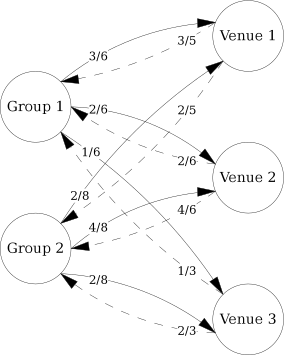
\includegraphics[width=5.5cm]{figures/models/bhrscore-w3}}
   \centerline{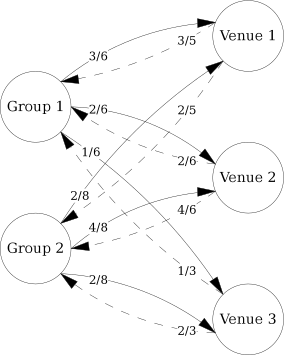
\includegraphics[width=5.2cm]{figures/models/bhrscore-w3}}
   \caption{Markov chain for an example with 2 research groups and 3 publication venues.}
   \label{fig:ex1-MC}
\end{figure}

From Figure \ref{fig:ex1-MC}, Group 1 published $3$ papers in venue $\mbox{v}_1$, $2$ papers in venue $\mbox{v}_2$, and $1$ paper in venue $\mbox{v}_3$. The number of publications of Group 1 is $6$. Venue $\mbox{v}_1$ receives $3$ papers of Group 1, and 2 papers of Group 2. The fractions of publications from groups to venues and from venues to groups are the edge weights. We have:
\[
\bP =
\left[
\begin{array}{c c | c c c }
0            &0             &3/6       &2/6         &1/6    \\
0            &0             &2/8       &4/8         &2/8    \\
\hline
3/5          &2/5           &0         &0           &0       \\
2/6          &4/6           &0         &0           &0       \\
1/3          &2/3           &0         &0           &0       \\
\end{array}
\right].
\]

This stochastic matrix corresponds to the Markov chain displayed in Figure~\ref{fig:ex1-MC}, which can be immediately aggregated to a two-state Markov chain, yielding:
%
\[
\bP^\prime = 
\left[
\begin{array}{c c }
0.467   &0.533 \\
0.400   &0.600
\end{array}
\right],
\]
\noindent which is the stochastic matrix we use in the solution of Equation (\ref{eq:top-rank}). (Recall that the dimension of $\bP^\prime$ is $T \times T$ and, as such, much smaller than that of $\bP$ for real size problems.) Solving Equation (\ref{eq:top-rank}) and applying Equation~\eqref{eq:venue-rank}, we obtain the ranking for the three venues: 
\begin{equation}
\bgamma\bkt{T} = \langle 0.36, 0.43, 0.21 \rangle.
\end{equation}

Venue $\mbox{v}_2$ has the highest rank, followed by $\mbox{v}_1$, and then by $\mbox{v}_3$. We remark that the individual values give the {\em relative reputation} of each publication venue. 
%
Then, we can apply Equation (\ref{eq:pscore}) to compute the P-score of each entity in the reputation graph.



%% Flow equations
\subsection{Flow Equations}\label{sec:flow-equations}

We recursively define the reputation of sources in terms of the reputation of targets, and the reputation of targets in terms of the reputation of sources. Specifically, the reputation $\gamma_s$ of a source $s$ is defined as:
\begin{align}
  \gamma_s = \sum_{t \in T} (1-d\bkt{T}).\bP_{ts}\bkt{TS} \gamma_t + \sum_{s' \in S} (d\bkt{S}).\bP_{s's}\bkt{SS} \gamma_{s'}.\label{eqn:gs}
\end{align}

In the summation, $\bP_{ts}\bkt{TS}$ is the transition probability from $t$ to $s$, given by $\bP_{ts}\bkt{TS} = n_{ts} / n_t$, where $n_{ts}$ is the number of edges running from $t$ to $s$ and $n_t$ is the total number of edges running from $t$. Finally, $\gamma_t$ is the reputation of target $t$, defined recursively as:
\begin{align}
  \gamma_t = \sum_{s \in S} (1-d\bkt{S}).\bP_{st}\bkt{ST} \gamma_s + \sum_{t' \in T} (d\bkt{T}).\bP_{t't}\bkt{TT} \gamma_{t'}.\label{eqn:gt}
\end{align}

Similarly, in the summation, $\bP_{st}\bkt{ST}$ is the transition probability from $s$ to $t$, given by $\bP_{st}\bkt{ST} = n_{st} / n_s$, where $n_{st}$ is the number of edges running from $s$ to $t$ and $n_s$ is the total number of edges running from $s$. Recall that $\gamma_s$ is the reputation of source $s$, defined according to Equation~\eqref{eqn:gs}.



%% Reputation
Reputation is a widespread notion in society, albeit an arguably ill-defined one. In general, the reputation of an entity reflects the public perception about this entity developed over time \cite{ribas2015random}. This public perception may be either good or bad, and touches a variety of aspects that may impact the identity of the entity before the public, such as its competence, integrity and trustworthiness. Moreover, the reputation of an entity can change rapidly following an event in which the entity is involved, by means of word-of-mouth dissemination -- whether traditional or electronic. As a result, reputation has been subject of professional management by public relations departments as well as of collective management by members of online communities, such as question-answering forums and online marketplaces \cite{hutton2001prr}.

%% Reputation-flows
In contrast to the aforementioned works, we use random walks to model the \textit{transference} of reputation from \textit{multiple} reference sources to selected targets in a reputation graph, as discussed in our previous work \cite{ribas2015random}. In order to validate our model, we instantiated it in an academic search setting by using research groups as reputation sources and publication venues as reputation targets. Moreover, while previous approaches have exploited multiple ranking signals, we demonstrated the power of the notion of reputation transfer by relying on publishing behavior as the only reputation signal.

%% Reputation-flows in Academia
Here we briefly discuss the instantiation of our conceptual framework of {\em reputation flows} in the academic context to model the transference of reputation between authors, papers, research groups and publication venues. The relations between these scientific entities may be captured through distinct metrics and, as far as we know, the most important ones (including citation-based metrics) fit well in our conceptual framework. In our experiments, we study how the reputation of a reference set of research groups is propagated to the venues they publish in and to other individual researchers by applying the concept of reputation flows. In this conceptual framework, publication venues are aggregations of papers and research groups are aggregations of authors, as shown in Figure~\ref{fig:groups-venues}. These aggregations are sufficient to establish core relations that allow ranking these entities.

%% One of the goals
One of the goals of this work is to find a fair and trustworthy way to rebalance these academic rankings in the context of sub-areas. 


%%  CAPES and AUTHORS CLASSIFICATION
In particular, we present in Table~\ref{tab:cnpq-levels} the current distribution of Brazilian researchers according to CNPq productivity levels in CS. This distribution is the result of an evaluation process quite similar to the aforementioned assessment of reputation made by the NRC. The table shows that there are just 390 CS researchers in all of the Brazil, out of many thousands, who receive an individual research grant from CNPq. 
%
To compute this distribution, an important rule is applied: regardless the metric used to rank researchers, there is a percentage limit for the number of authors in each productivity level, except the last one (level 2). This limitation applies to the whole area of CS, without considering the specificities of each of its subareas. One can see that independently of the academic metrics used, some subareas of CS have intrinsic disadvantages in this classification. These problems motivate our current work on this dissertation.

% cat bolsistas_produtividade.tsv | awk '{print $2}' | sort | uniq -c
\begin{table}[htbp]
\centering \small
\caption{Distribution of researchers in CNPq productivity levels in Computer Science (CS) and in all areas of science}
\label{tab:cnpq-levels}
\begin{tabular}{ccc}
\\
\toprule
Level & \multicolumn{2}{c}{Researchers} \\ %\cline{2-3}
      & CS & All Areas \\ 
\midrule
%SR   & 0 & 91 \\
1A &  23 (5.9\%) & 1320 (9.2\%) \\
1B &  22 (5.6\%) & 1308 (9.1\%) \\
1C &  31 (7.9\%) & 1376 (9.6\%) \\
1D &  70 (17.9\%) & 2386 (16.7\%) \\
2  & 244 (62.6\%) & 7933 (55.4\%) \\
\midrule
%Total & 390 & 14414 \\ % with SR
Total & 390 & 14,323 \\ % without SR
\bottomrule
\end{tabular}
\end{table}


%% Our approach ICTIR
In \cite{ueda17ictir}, we tackled the problem of both identifying the most important venues of a subarea in CS and rank US research groups based on this information, in a semi-automatic fashion. We showed that significant differences appears in rankings of graduate programs if we take the CS subareas into account. Those differences provide valuable information for decision making by funding agencies, department chairs, and undergraduate students searching for research departments, for instance.

%% Related intro
Several metrics for quantifying the reputation of academic entities have been proposed, including citation-based metrics, machine learning techniques, and Markov processes. Some of these metrics (e.g. H-index \cite{hirsch2005} and Impact Factor~\cite{garfield1955}) have been used by prestigious institutions, from academic search engines to government funding agencies to assess the reputation of authors, research groups, and publishing venues from the perspective of the broad areas of knowledge (e.g. Computer Science, Physics, Mathematics, Statistics, Chemistry, and so on). 



Figure and Table example
\begin{figure}[t]
    \centering
    \includegraphics[width=\linewidth]{fig/data-management}
    \caption{Uma figura de exemplo.}
    \label{fig:exemplo}
\end{figure}

\begin{table}[t]
    \caption{Uma tabela de exemplo.}
    {\centering
    \begin{tabular}{lcr} \toprule
    \emph{Left-aligned} & \emph{Centered} & \emph{Right-aligned} \\ \midrule
    Lorem ipsum & dolor sit & amet \\
    consectetur adipisicing & elit, sed do eiusmod & tempor \\
    incididunt ut & labore et dolore & magna aliqua. \\ \bottomrule
    \end{tabular}\par
    }
\end{table}
